\documentclass[graphics]{beamer}

\usepackage{graphicx}
\usepackage{verbatim}
\usepackage{wrapfig}
\useoutertheme{shadow}
%\usecolortheme{orchid}
\usecolortheme{seahorse}


% math commands
\newcommand{\be}{\begin{eqnarray}}
\newcommand{\ee}{\end{eqnarray}}
\newcommand{\beq}{\begin{equation}}
\newcommand{\eeq}{\end{equation}}
\def\simless{\mathbin{\lower 3pt\hbox
      {$\rlap{\raise 5pt\hbox{$\char'074$}}\mathchar"7218$}}}
\def\simgreat{\mathbin{\lower 3pt\hbox
      {$\rlap{\raise 5pt\hbox{$\char'076$}}\mathchar"7218$}}} %> or of order

% variables

\def\toonscale{0.45}
\def\mboxy#1{\mbox{\small #1}}


\begin{comment}
\AtBeginSection[]{
  \frame{
    \frametitle{Outline}
    \tableofcontents[currentsection]
  }
}
\end{comment}

\title{Astrophysical HPC
}
\subtitle{}
\author[U. Pen]{\textcolor{green}{Ue-Li Pen, and many collaborators
}
\\[8mm] 
}
\date{May 16, 2018}


\begin{document}

\frame{
\begin{picture}(320,250)
\put(-50,-130){
\includegraphics[width=5.5in]{Figures/delta_nu_sim.pdf}}
\end{picture}
\vspace{-3in}
\titlepage
}

%\section*{Introduction}
\section{Astrophysics: challenging the universe
}

\begin{comment}
  \subsection{Outline}

  \frame{
    \frametitle{Outline}
    \tableofcontents
  }
\end{comment}

  \frame{
\vspace{-0.5in}
    \frametitle{Challenge}
    \begin{itemize}
        \item HPC is the laboratory for controlled experiments
        \item small particles, big challenges: cosmic neutrino
          background (C$\nu$B)
        \item New telescopes, big data: CHIME, ARO, VLBI
        \item Unique opportunities in Ontario: Academics, telescopes, companies
        \item Industrial bridges: AMD, IBM, Thoth, SkyWatch, etc.
        \item platforms: McKenzie, GPC, BGQ, FPGA, GPU, TH2, Niagara
    \end{itemize}
  }
  \frame{
    \frametitle{Non-linear dynamics}
    \begin{itemize}
        \item 2015 Nobel prize for Art McDonald at Queens proved
          neutrinos have mass
        \item absolute mass scale testable in the universe
        \item non-linear but clean dynamics
        \item supercomputer to the rescue!
    \end{itemize}
\vspace{-0.1in}\hspace{.3in}
\includegraphics[width=2.2in]{Figures/th2photo.jpg}
}
  \frame{
    \frametitle{Movie}
    {\tt http://cita.utoronto.ca/\~\,haoran/thnu/movie.html}
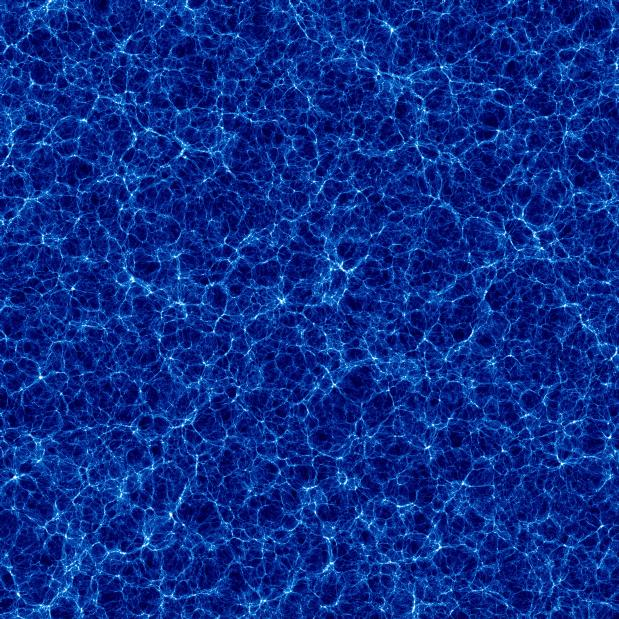
\includegraphics[width=4.2in]{Figures/thnucdmlowres.jpg}
}
  \frame{
    \frametitle{Differential clustering}
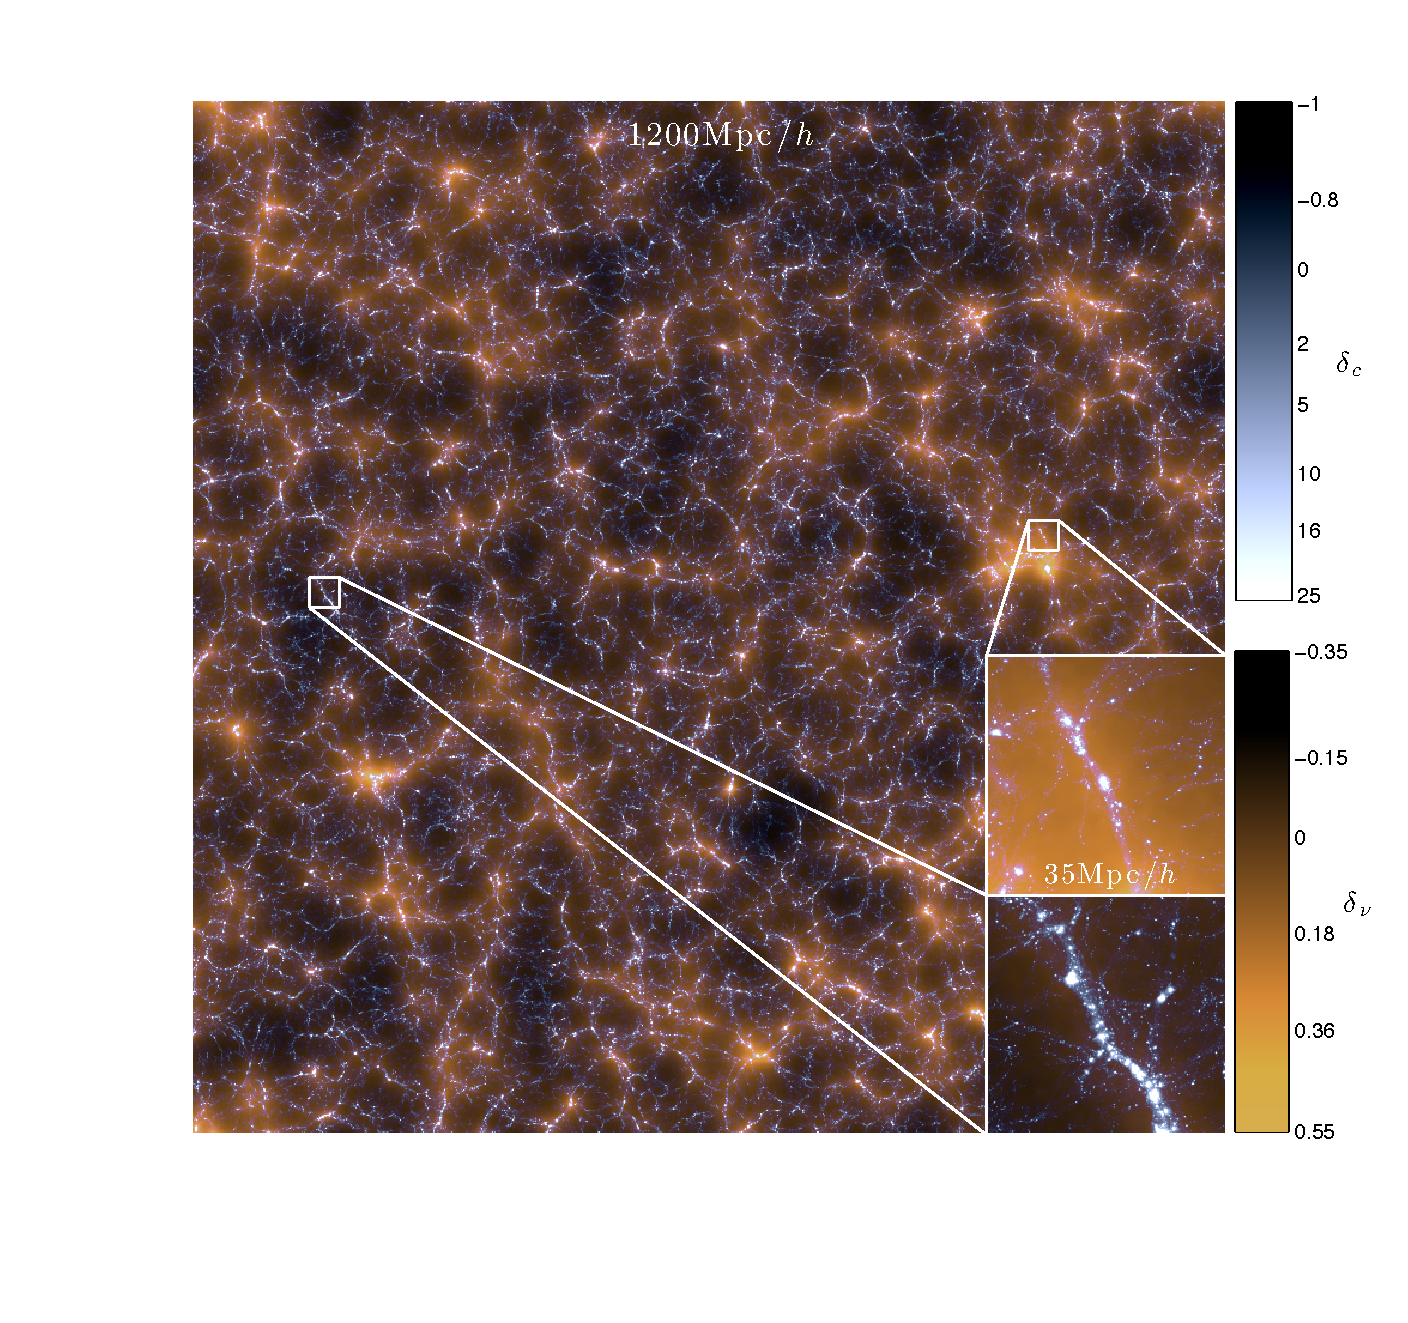
\includegraphics[width=3.5in]{Figures/cnudiff.pdf}
}


  \frame{
\vspace{-0.5in}
    \frametitle{Industrial Bridges}
    \begin{itemize}
        \item AMD Markham labs (formerly ATI)
        \item joint development of CHIME GPU correlator: low precision fixed
          point DSP, 7 PFLOP (FP32) machine developed and assembled at UofT,
          deployed in Penticton, BC
        \item hardware and software of immediate application to
          machine learning
        \item SOSCIP 
    \end{itemize}
\vspace{-0.01in}\hspace{.3in}
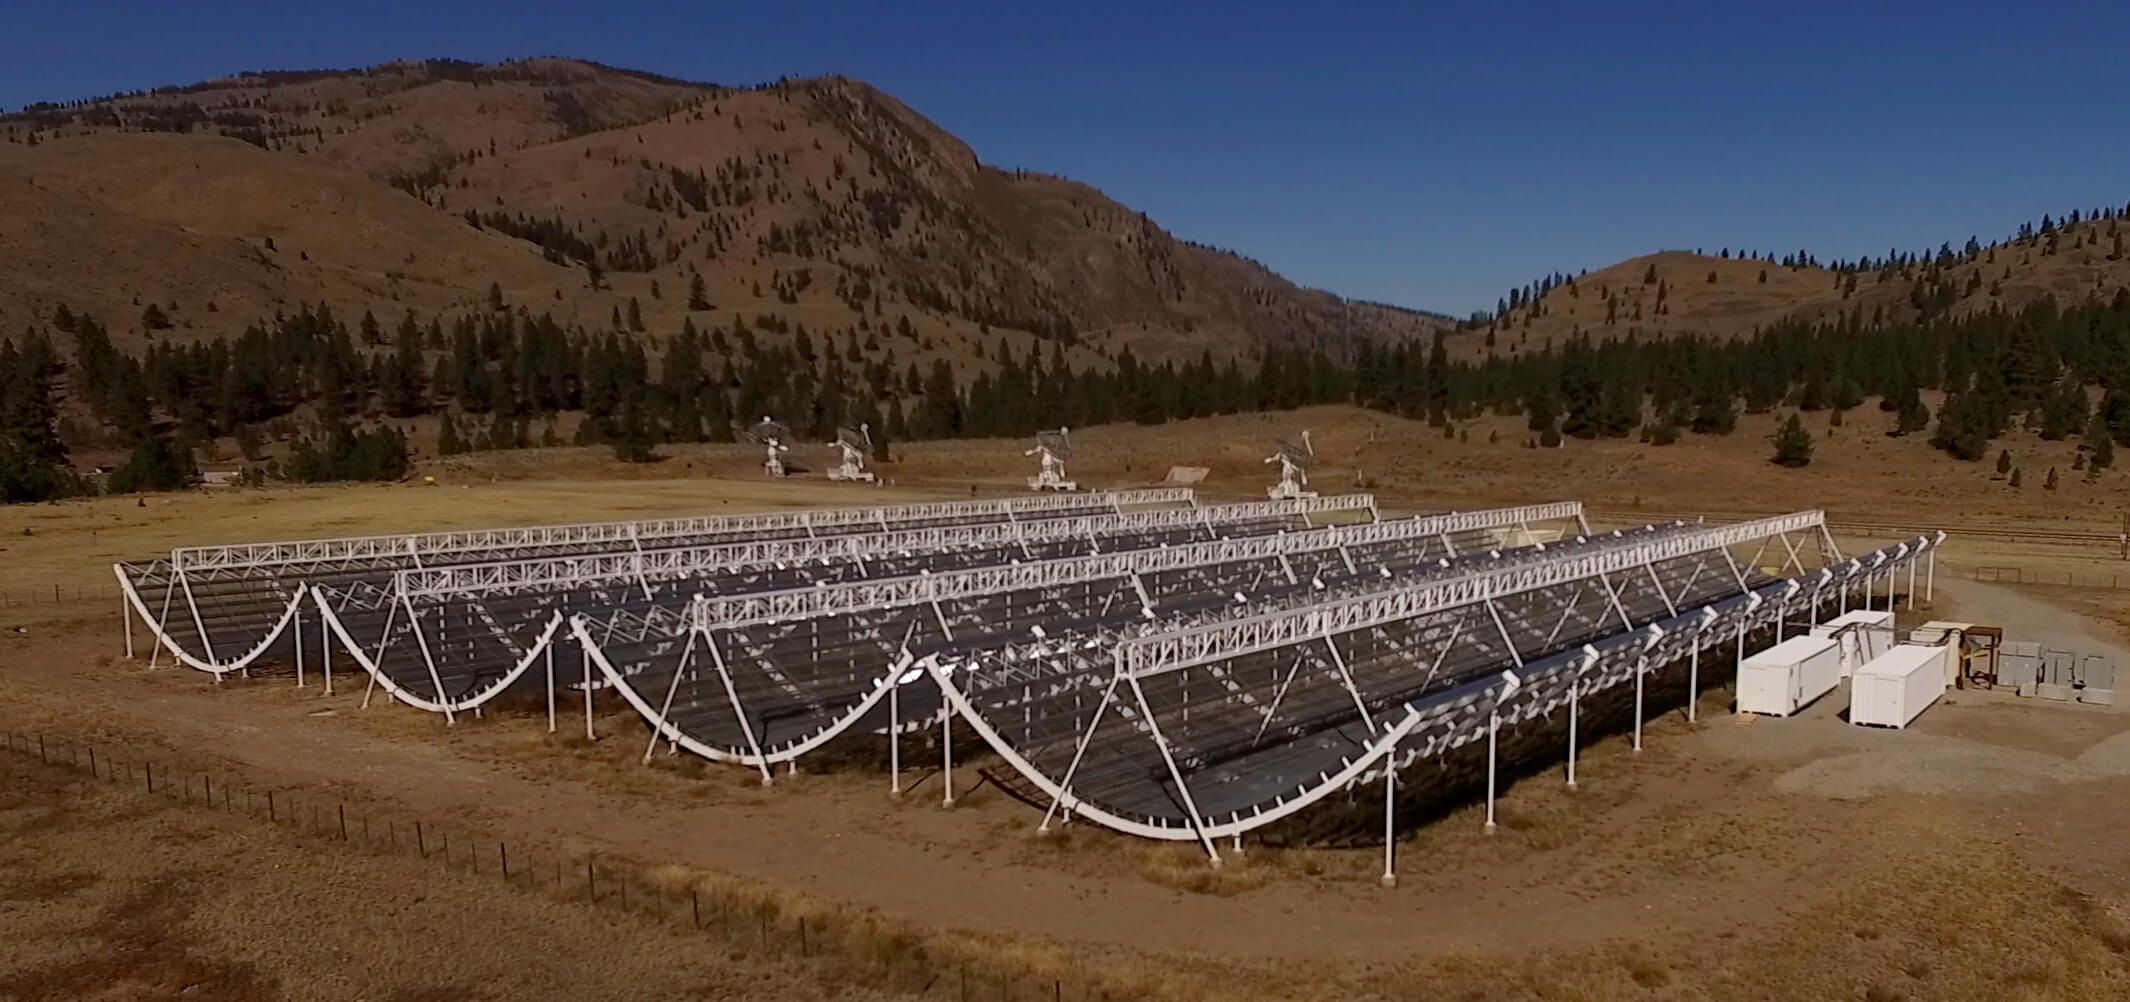
\includegraphics[width=2.2in]{Figures/chime.jpg}
  }


  \frame{
\vspace{-0.5in}
    \frametitle{Reflections}
    \begin{itemize}
        \item high performance custom codes quickly adaptable to new platforms
        \item 8-bit fixed point rennaisance: N-body, astrophysical
          signal processing, Machine Learning
        \item heterogenous future: GPU's, FPGAs
        \item  
    \end{itemize}
\vspace{-0.1in}\hspace{.3in}
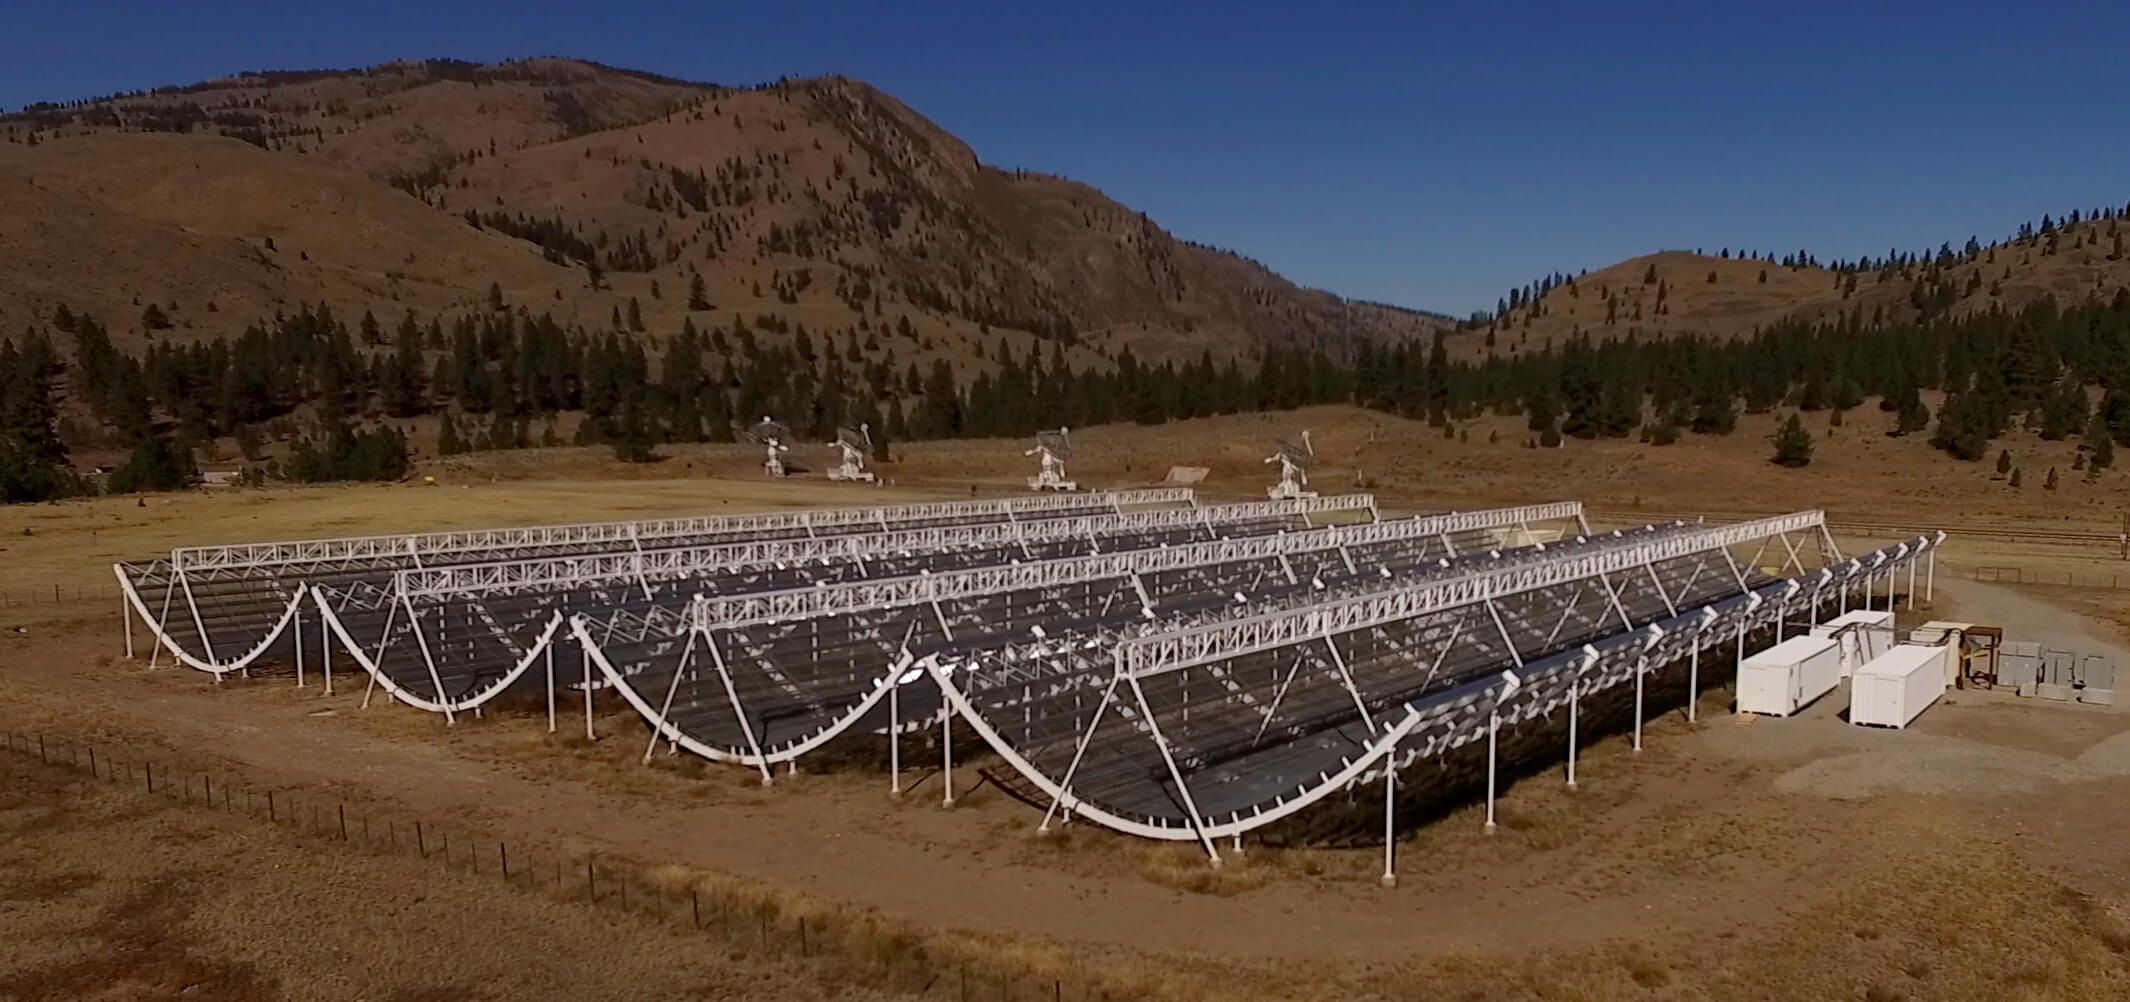
\includegraphics[width=2.2in]{Figures/chime.jpg}
  }


\end{document}
